% This is LLNCS.DEM the demonstration file of
% the LaTeX macro package from Springer-Verlag
% for Lecture Notes in Computer Science,
% version 2.4 for LaTeX2e as of 16. April 2010
%
\documentclass{llncs}
%
\usepackage{makeidx}  % allows for indexgeneration
\usepackage{epsfig} % allows encoding PostScript images
\usepackage{graphicx}
\usepackage{amsmath}
\usepackage{subfigure}
%
\begin{document}
%
\frontmatter          % for the preliminaries
%
\pagestyle{headings}  % switches on printing of running heads
\mainmatter              % start of the contributions
%
\title{Fiber feature map based landmark initialization for highly deformable DTI registration}
\author{COMP 992 Report by Ravikiran Janardhana$^{1}$ \\ \vspace{2mm} Co-Authors: Aditya Gupta$^{2,4}$, Matthew Toews$^{3}$, Yogesh Rathi$^{3}$, John Gilmore$^{4}$, Maria Escolar$^{2}$, Martin Styner$^{1,4}$}

\institute{$^{1}$Dept Computer Science, University of North Carolina, Chapel Hill, $^{2}$Dept Pediatrics, University of Pittsburgh, PA, USA; ${^3}$Harvard Medical School, Boston MA; ${^4}$Dept Psychiatry, University of North Carolina, Chapel Hill.}


\maketitle              % typeset the title of the contribution

% begin abstract

\begin{abstract}
This paper presents a novel pipeline for the registration of diffusion tensor images (DTI) with large pathological variations to normal controls based on the use of a novel feature map derived from white matter (WM) fiber tracts. The research presented aims towards an atlas based DTI analysis of subjects with considerable brain pathologies such as  tumors or hydrocephalus. In this paper, we propose a novel feature map that is robust against variations in WM fiber tract integrity and use these feature maps to determine a landmark correspondence using a 3D point correspondence algorithm. This correspondence drives a deformation field computed using Gaussian radial basis functions(RBF). This field is employed as an initialization to a standard deformable registration method like demons. We present early preliminary results on  the registration of a normal control dataset to a dataset with abnormally enlarged lateral ventricles affected by  fatal demyelinating Krabbe disease. The results are analyzed based on a regional tensor matching criterion and a visual assessment of overlap of major WM fiber tracts. While further evaluation and improvements are necessary, the results presented in this paper highlight the potential of our method in handling registration of subjects with severe WM pathology.

\keywords{fiber feature map, 3D point correspondence, DTI, large deformation fields}
\end{abstract}

% end abstract


% begin introduction
% end introduction

\section{Introduction}
\label{sec:intro}
Diffusion tensor imaging (DTI) has proven especially of value in clinical studies of white matter (WM) integrity in the developing brain. In this paper, we focus on the application of DTI in a natural history study of a particularly devastating WM demyelinating disease called Krabbe \cite{Escolar09}. Previous studies show that neonates with infantile Krabbe disease have lower fractional anisotropy (FA) across the corpus callosum and along the DTI fiber bundle of internal capsules (IC) when compared with healthy age-matched controls \cite{Guo01}. Based on the above findings, atlas based fiber tract analysis is used for analyzing DTI of Krabbe subjects \cite{Goodlett06}. For accurate analysis of WM fiber tracts it is crucial to establish a registration based voxel-wise correspondence between a normal control and the Krabbe subjects. 

In addition to the pathological WM integrity, untreated infantile Krabbe cases may develop significantly enlarged lateral ventricles, a condition similar to hydrocephalus. The enlargement of the lateral ventricles push the fiber tracts against the skull, making it very difficult to analyze these images with an atlas based methodology. In our studies, the clinicians are interested to investigate fiber tracts based DTI analysis in such natural history cases as this reveals crucial information about disease progression.

The research in this paper is a step towards the analysis of these fiber tracts. The paper presents a method to determine point correspondences between the subject case and the normal control automatically by computing novel feature maps from the DWI data. These feature maps highlight the crossing fiber regions and are based on voxel-wise fiber density and entropy computations. The point correspondences are used to determine a deformation field via Gaussian radial basis functions (RBF) \cite{Mike99}. This deformation field  is then used to initialize a standard registration method. The results are presented on a Krabbe subject with particularly abnormal enlarged ventricles to highlight the potential of the proposed approach.

The main contributions of this paper include a novel feature map determined from DWI data, which highlights the single and crossing fiber geometry, while being robust against variations in WM fiber tract integrity, a feature desirable in many WM demyelinating pathologies. Also this paper proposes a novel registration pipeline, which uses this feature map alongside a 3D correspondence algorithm and a Gaussian RBF to initialize standard registration algorithms to handle high anatomical deformations.

\section{Methodological Background}
\label{sec:methodBackground}
Registration of DTIs is particularly challenging, as DTI data is multi-dimensional and the tensor orientations after image transformations must remain consistent with the anatomy. Prior to the development of full tensor based registration methods, DTI registration was performed with traditional image registration algorithms on scalar images derived from the DTI. The performance of scalar and full tensor registration algorithms are compared for Krabbe neonates \cite{Wang11} and the full tensor based DTI-TK \cite{Zhang06} method showed the most accurate performance. % followed by the demons algorithm on the scalar fractional anisotrophy (FA) images.

The major drawback when using DTI derived FA scalar map in the registration of WM demyelinating pathologies is that the FA values are majorly affected by the pathology. While intensity normalization approaches have been employed to reduce the impact of this issue, major pathologies cannot be handled in this way. This drives the motivation of our proposed work towards a feature map that is robust against variations in WM fiber tract integrity. Several authors have used other DTI derived scalar maps such as radial diffusivity (RD), mean diffusivity (MD) or even multichannel registration \cite{Alexand99} with several of these feature maps. But again these methods rely on properties derived from the fiber tracts, which may be an issue in pathologies such as Krabbe with large structural variations. The motivation of our proposed feature map is to highlight voxel-wise fiber geometry features such as crossing fiber and single fiber situations, which can be largely independent of the fiber tract properties and thus be used  as the driving force for registration. The next section discusses the methodology behind generating these feature maps, the point correspondence, initial deformation field and the final deformation.


\section{Method}
\label{sec:method}
The first part of this section describes the steps involved in generating the novel feature map from DWI data. The second part describes the algorithm for determining the point correspondence on these feature maps. This is followed by a description on using the point correspondences to determine an initial deformation field through Gaussian RBF. Finally the steps involved in using this deformation field as an initialization to a standard registration algorithm are discussed.

%
\subsection{Feature Map Generation}
\label{subsec:FeatureMap}
%
In this section, we present the steps involved in generating the feature map from the raw diffusion weighted image (DWI) and the image mask. First, we perform a 2-tensor unscented kalman filter based tractography \cite{malc10} in order to obtain the fiber tracts image. Once the fiber tracts have been generated, we compute two main features namely, number of fiber segments per voxel and entropy of fiber orientations per voxel.  We normalize and combine these two features in order to develop the feature image. The following sections describe each step of the feature map generation in detail.

%
\subsubsection{Fiber Tracts Generation}
%
The fiber tracts are generated from the raw DWI image and the image mask by performing a 2-tensor unscented kalman filter (ukf) based tractography. Unlike many of the existing techniques, in ukf-based tractography, fiber tracking is formulated as causal estimation; at each step of tracing the fiber, the current estimate of the signal is guided by the previous. To do this, the signal is modeled as a discrete mixture of Watson directional functions and tractography is performed within a filtering framework. Starting from a seed point, each fiber is traced to its termination using an unscented Kalman filter to simultaneously fit the signal and propagate in the most consistent direction. Despite the presence of noise and uncertainty, this provides an accurate estimate of the local structure at each point along the fiber. The in-depth details of the tractography can be found in \cite{malc10}.  

While generating the fiber tracts, we can configure various parameters, the most important ones being number of seeds per voxel, seed FA limit, minimum FA to continue tractography and branching factor. Figure \ref{fig:parameterConfig} shows the fiber tracts generated for different parameter configurations. Based on visual assessment of the fiber tracts generated, for our experiments, we configured number of seeds per voxel as 8, seed FA limit as 0.18, minimum FA to continue tractography as 0.12 and suppressed branching. The minFA and seedFA are set very low as the FA values are very low in Krabbe cases.

\begin{figure}
    \centering
    \subfigure[]{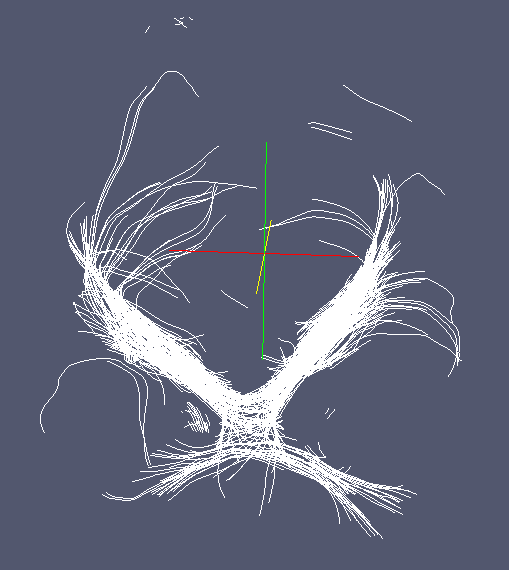
\includegraphics[height=0.20\textheight,width=0.30\textwidth]{images/ukf-a.png}\label{fig:ukfA}}
    \subfigure[]{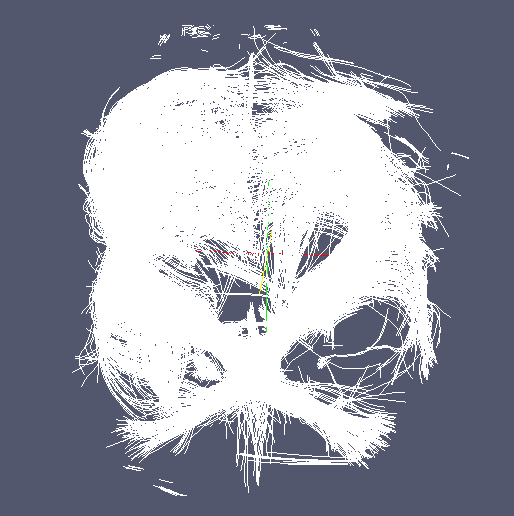
\includegraphics[height=0.20\textheight,width=0.30\textwidth]{images/ukf-b.png}\label{fig:ukfB}}
    \subfigure[]{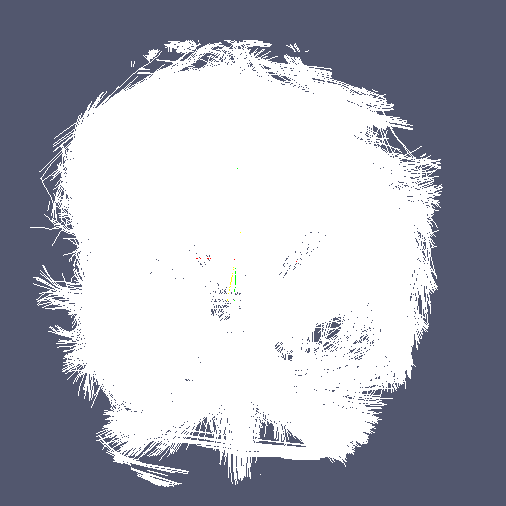
\includegraphics[height=0.20\textheight,width=0.30\textwidth]{images/ukf-c.png}\label{fig:ukfC}}
    \caption{The figures show the fiber tracts generated at different parameter configurations. (a) seedFA = 0.30, minFA = 0.25, seedsPerVoxel = 1, (b) seedFA = 0.20, minFA = 0.20, seedsPerVoxel = 4, (c) seedFA = 0.18, minFA = 0.12, seedsPerVoxel = 8.}
    \label{fig:parameterConfig}
\end{figure}

%
\subsubsection{Fiber Segments per voxel}
%
In this step, we traverse through all the fiber segments in the fiber tracts generated and identify which voxel a particular fiber segment belongs to and increment its counter by one.  The result of this step is an image where the value at a particular voxel indicates the number of fiber segments it contains and thus indicates the density of fibers at that voxel.

%
\subsubsection{Entropy of Fiber Orientations}
%
In order to compute the entropy of fiber orientations at a particular voxel, we first need to define what is the fiber orientation at a voxel. Consider the below example in Figure \ref{fig:histogram}, where a single fiber passes through the fiber points p1, p2 and p3 at a particular voxel. The fiber orientation at a fiber point is defined as the direction of the tangent joining its neighboring fiber segment points. At the boundary fiber points, the fiber orientation is defined as the direction of the line connecting it to the previous or subsequent fiber point. The fiber orientation at a voxel can now be defined as a tuple of fiber orientations at the fiber points contained in the voxel.

\begin{figure}
\centering
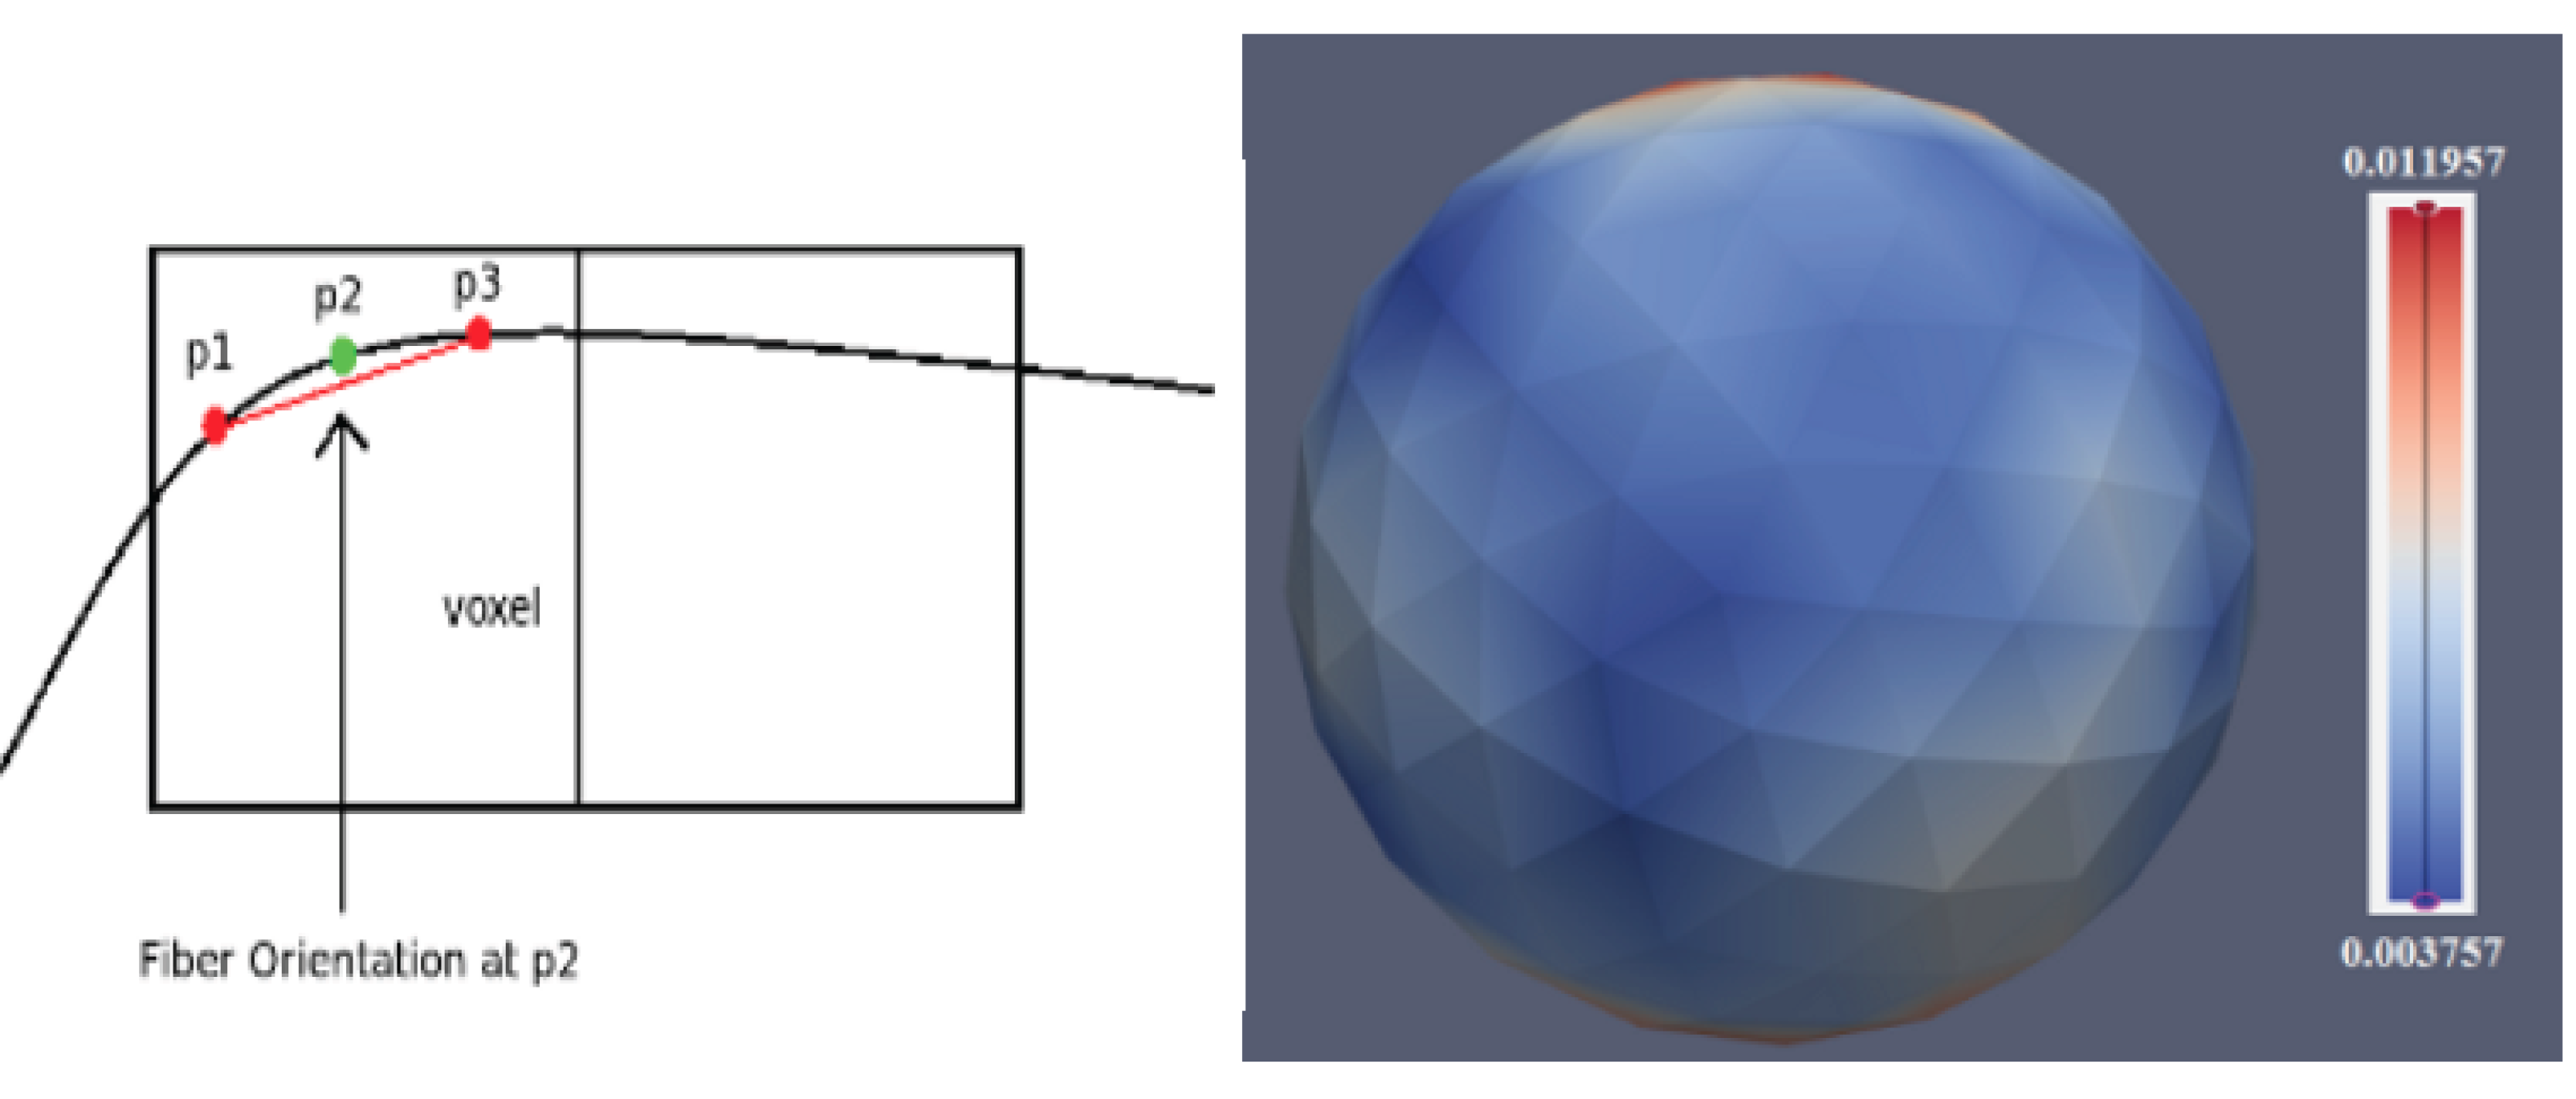
\includegraphics[width=1\columnwidth]{images/fiber_orientation_histogram.png}
\caption{Fiber orientation computed at a fiber segment point and the histogram representing the fiber orientations of a particular voxel on a unit sphere.}
\label{fig:histogram}
\end{figure}
%
The next step is to compute the histogram (see Figure \ref{fig:histogram}) of these fiber orientations at each voxel. This histogram computed is on a unit sphere which is subdivided into equal regions by fitting a platonic solid such as an icosahedron onto the surface of the sphere with a sub-division level of 6.  At the subdivision level of 6, we get 492 icosahedron vertices and given a fiber orientation, we approximate it to a particular icosahedron triangular face and add it to the icosahedron vertices using barycentric coordinate system in which the location of the fiber direction is specified as the center of mass, or barycenter, of masses placed at the vertices of a simplex i.e., a triangle in our case.

This histogram is then used to generate the entropy of fiber orientations. Entropy is a measure of disorder, or more precisely unpredictability.  For example, a series of coin tosses with a fair coin has maximum entropy, since there is no way to predict what will come next. A string of coin tosses with a coin with two heads and no tails has zero entropy, since the coin will always come up heads. Similarly if there is just a single track fiber, there is less unpredictability and hence lower entropy and if there are multiple fiber tracts and multiple fiber orientations, this means that there is more unpredictability and hence higher entropy. 
 
Using the histogram, we compute entropy of fiber orientations per voxel as below: 
 
\begin{equation}
H(X) = - \sum_{i=1}^n p(x_i) \log_{b} p(x_i) 
\end{equation}

where, \textit{H(X)} is the entropy of fiber orientation at a particular voxel, \textit{p(x$_{i}$)} is the probability of a fiber orientation to be \textit{x$_{i}$} and \textit{n} represents all possible fiber orientations. 

%
\subsubsection{Combining features to obtain Feature Map}
%
In order to obtain the feature map, we first normalize the two features namely fiber segments per voxel and entropy of fiber orientations per voxel by dividing each of these by their respective maximum. The feature map is then obtained by computing the square root of the product of normalized values of the two features.

%Equation
\begin{equation}
    F_i(X) = \sqrt {\frac{H_i(X)}{H_{max}(X)} * \frac{fs_i(X)}{fs_{max}(X)} }
\end{equation}

where \textit{F$_i$(X)}, \textit{H$_i$(X)} and \textit{fs$_i$(X)} are the feature map value, entropy of fiber orientations and the number of fiber segments at voxel \textit{i} respectively, \textit{$H_{max}(X)$} and \textit{$fs_{max}(X)$} are the maximum values of entropy of fiber orientations and number of fiber segments over the entire image. 

This feature map (see Figure \ref{fig:featureMap}) is certain to highlight the crossing fiber landmarks which can further be used for DTI registration.  If one examines the fiber segments per voxel image, it is bound to have higher intensities in those regions where there are large number of single fiber tracts and multiple fiber tracts and lower intensities in regions of fewer or no fiber tracts.  The entropy of fiber orientations image has higher intensities in regions of dispersed single fiber tracts and crossing fiber tracts (due to greater variation in fiber orientations) and lower intensities in uni-directional single fiber tracts or no fiber tracts regions. Hence, by combining these two, we can negate out the uni-directional single fiber tracts and no fiber tracts regions, thus highlighting the crossing fiber regions or landmarks.

\begin{figure}
    \centering
    \subfigure[]{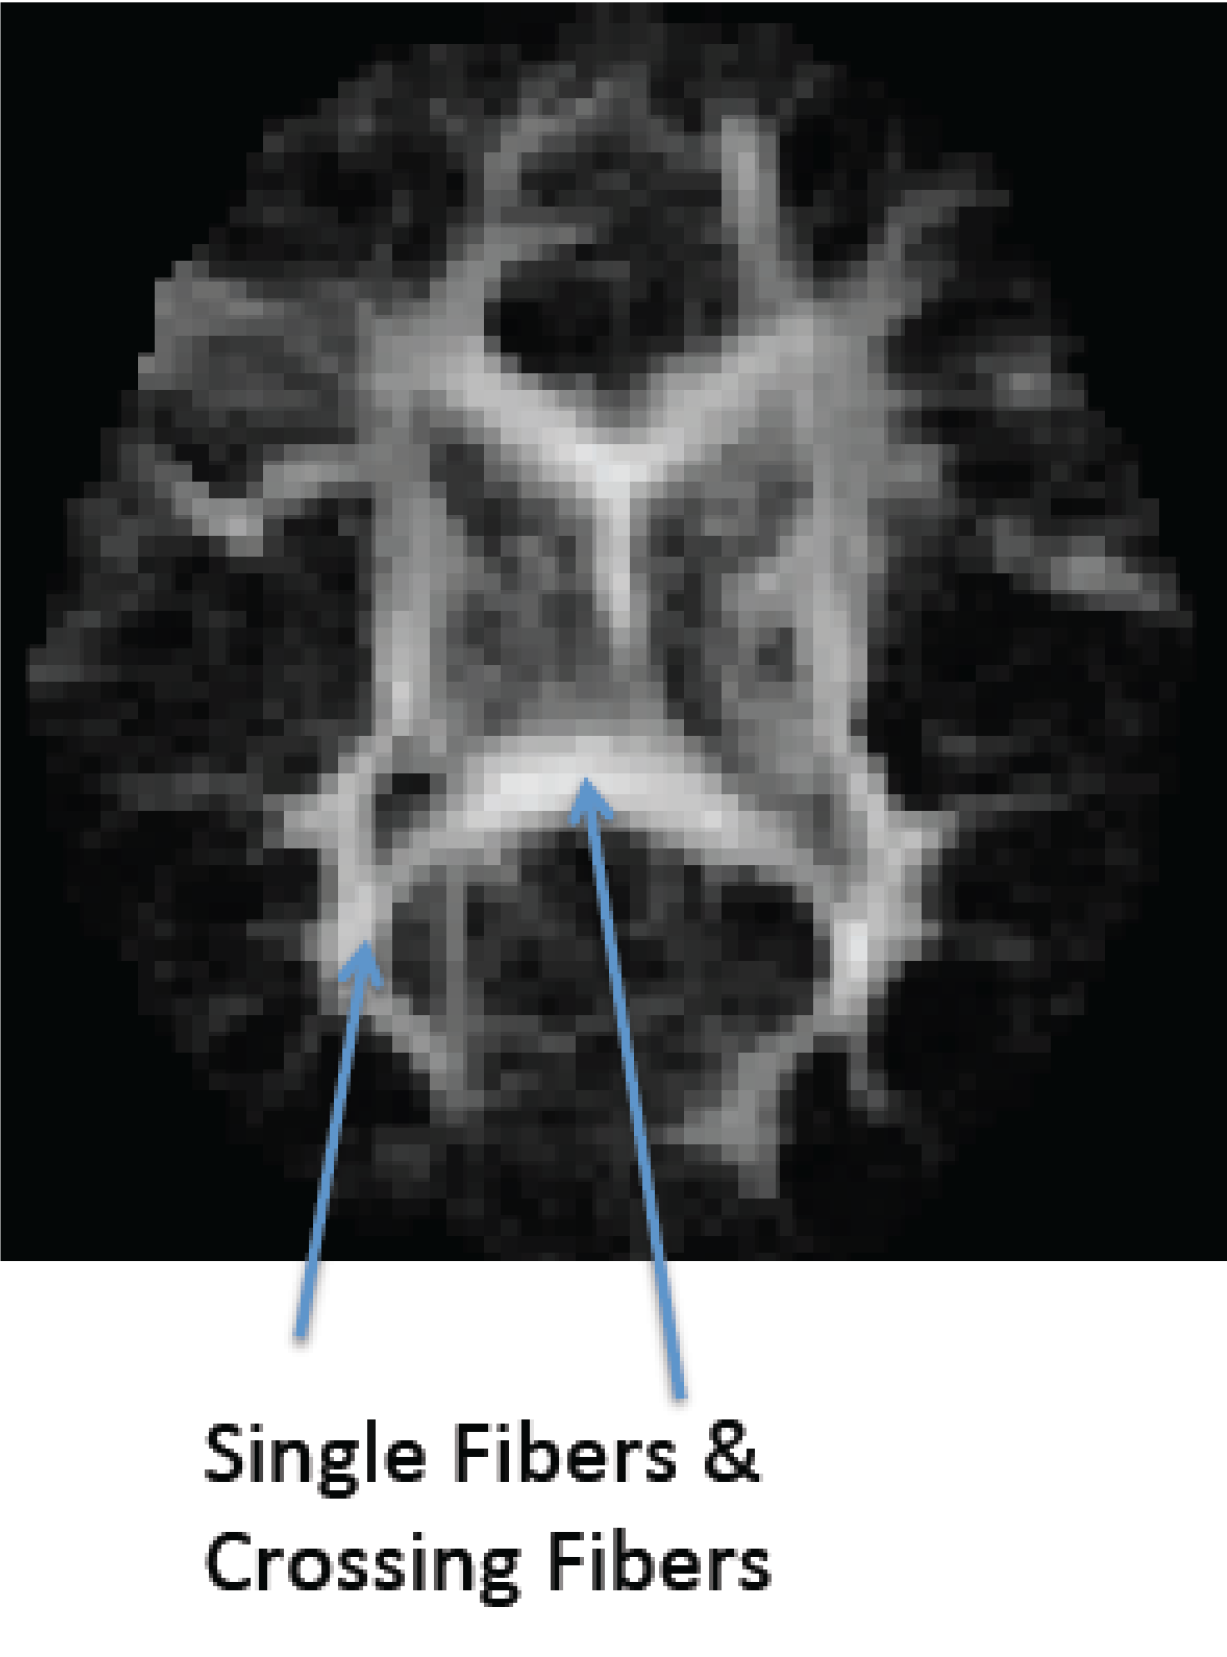
\includegraphics[height=0.30\textheight,width=0.30\columnwidth]{images/feature_map-a.png}\label{fig:featA}}
    \subfigure[]{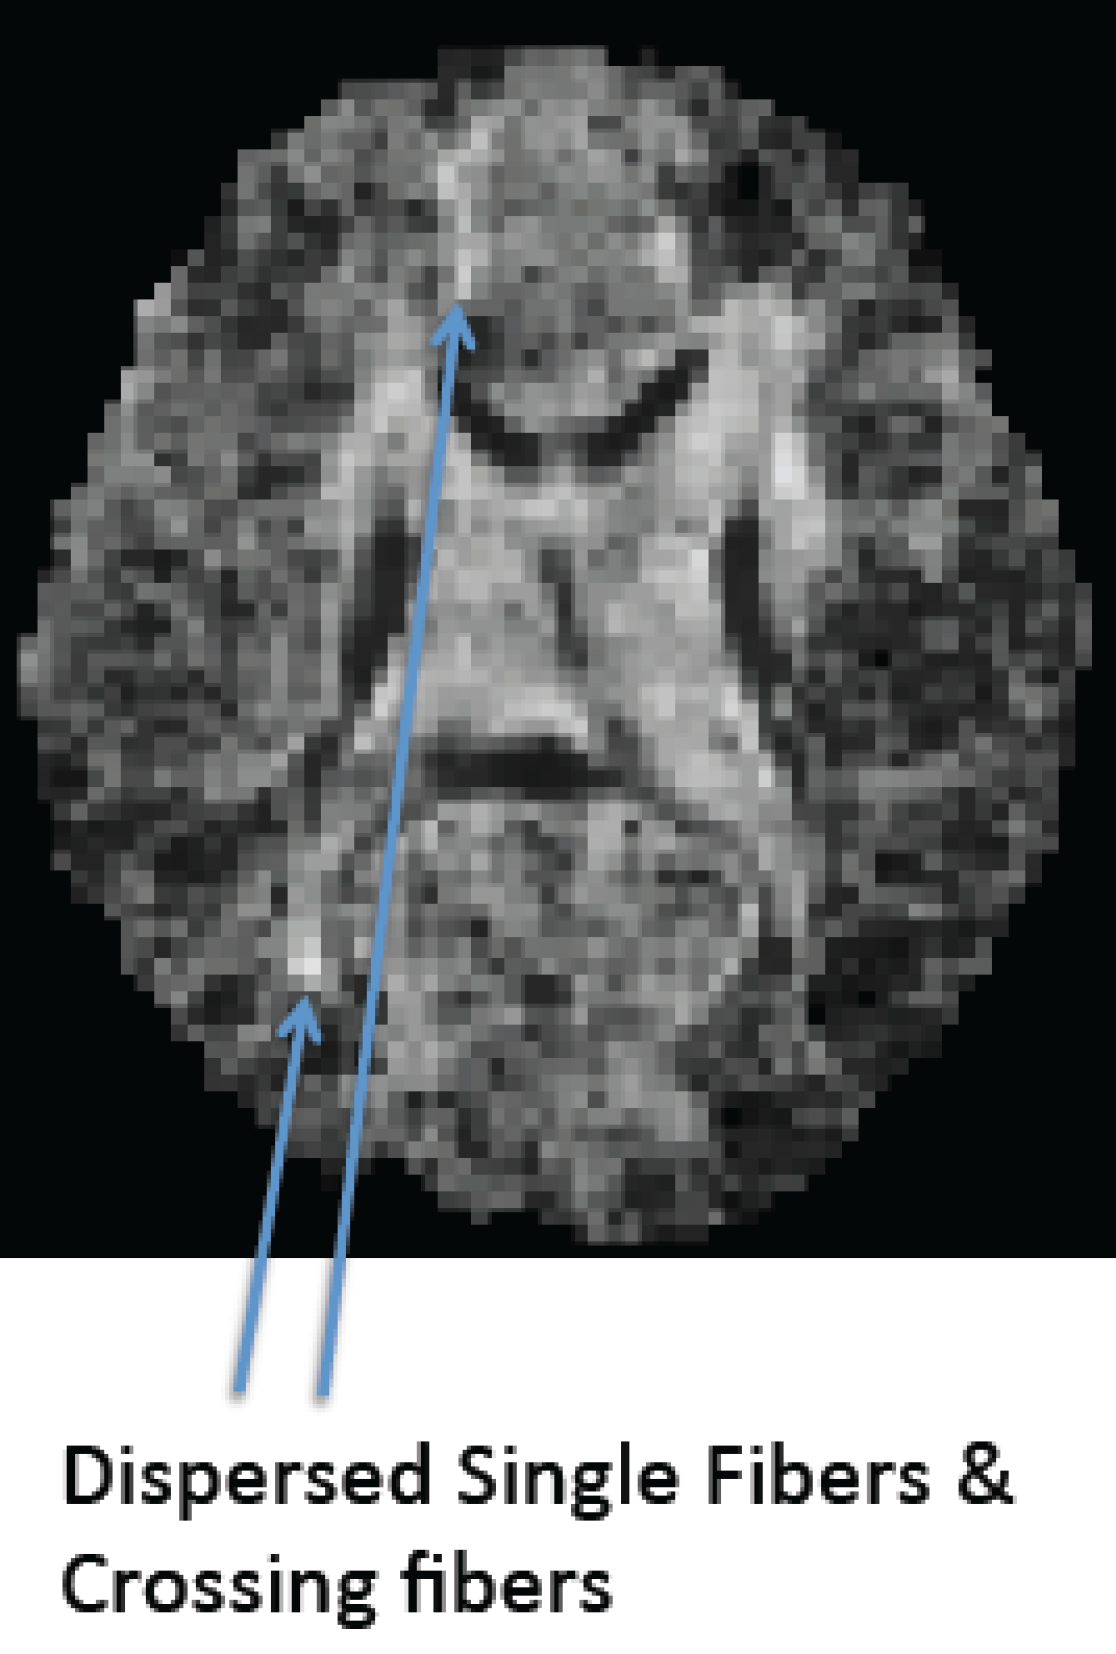
\includegraphics[height=0.30\textheight,width=0.30\columnwidth]{images/feature_map-b.png}\label{fig:featB}}
    \subfigure[]{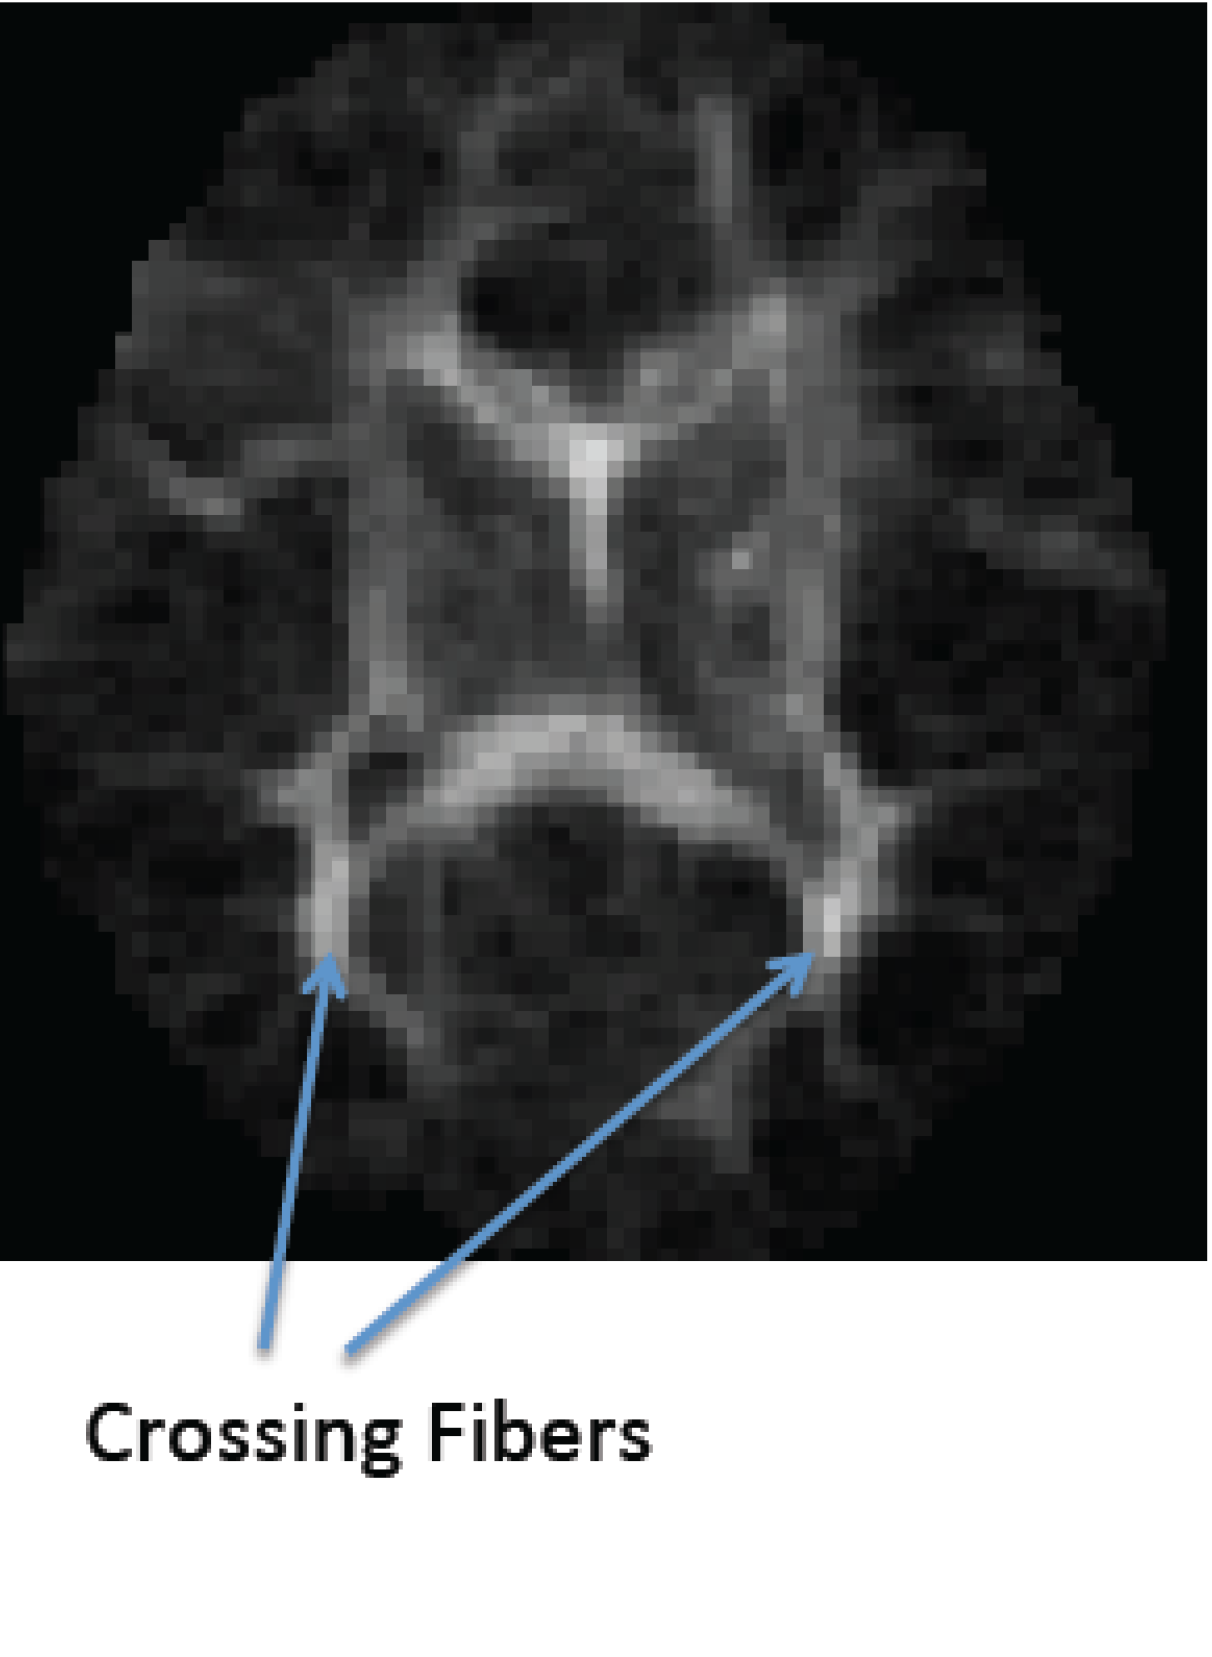
\includegraphics[height=0.30\textheight,width=0.30\columnwidth]{images/feature_map-c.png}\label{fig:featC}}
    \caption{Feature maps in normal control subject. (a) Fiber Segments per voxel image; (b) Entropy of fiber orientations per voxel image; (c) Combined feature map image. The regions with crossing fibers are marked with arrows and display a high intensity in the final feature map.}
    \label{fig:featureMap}
\end{figure}

%
\subsubsection{Note on Inconclusive features}
%
We also explored other features such as Earth Mover's Distance of Fiber distance histogram in hope of obtaining a pathology invariant feature map. The fiber distance was defined as the spherical distance between weighted individual fiber orientation to strongest fiber orientation at a particular voxel. However, the results produced were inconclusive and hence, we decided to not include it in the feature map.

\subsection{Landmarks with correspondence on feature maps}
\label{subsec:Correspondence}
Deformable intensity-based image registration methods employ local optimization methods that largely driven by distinctive image structure, i.e. corners or landmarks, and must be correctly initialized in order ensure convergence to correct solutions. Here, we achieve initialization from a set of robust image-to-image correspondences obtained via a 3D version of the scale-invariant feature transform (SIFT) matching technique of Lowe et al~\cite{Lowe:04}. The SIFT technique operates by identifying maxima in a difference-of-Gaussian (DoG) operator:
\begin{equation}
 \{x,y,z,\sigma\} = \underset{x,y,z,\sigma}{\mbox{local argmax}}\left\{|G(x,y,z,\sigma)-G(x,y,z,\kappa\sigma)|\right\},
\end{equation}

where $G(x,y,z,\sigma)$ represents the convolution with a Gaussian operator of variance $\sigma^2$ and $\kappa$ is a constant. Image regions centered on $x,y,z$ of size proportional to $\sigma$ are then cropped and spatially normalized via rescaling and reorientation to a local coordinate system~\cite{Allaire:08}, and encoded as an appearance descriptor. Image-to-image matching proceeds by computing nearest neighbors between features extracted in different images, based on the Euclidean distances of appearance descriptors. Note that due to spatial feature normalization, nearest neighbors can be computed despite arbitrary global similarity image transforms (i.e. translation, rotation and isotropic scaling). Finally, the Hough transform is applied to determine a set of correspondences that are inliers of a robust image-to-image similarity transform.

\begin{figure}
    \centering
    \subfigure[Normal Control]{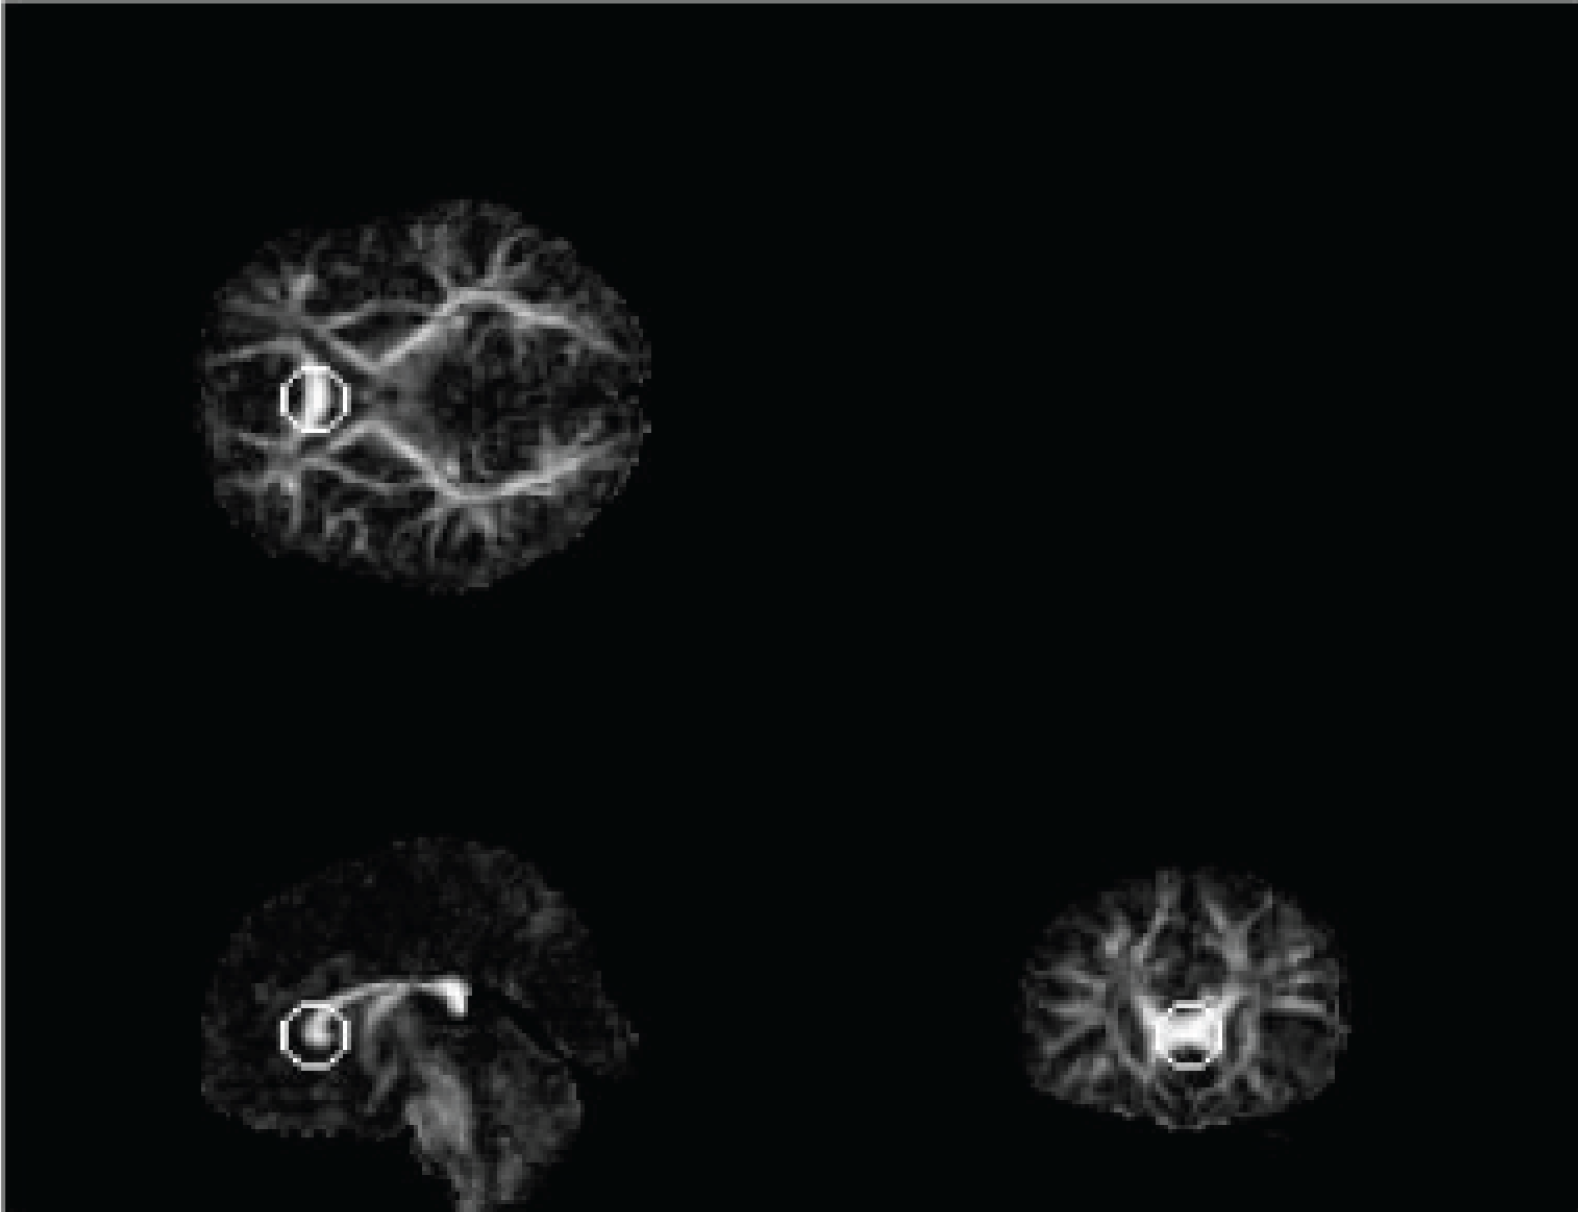
\includegraphics[height=0.33\textheight,width=0.49\columnwidth]{images/correspondence-a.png}\label{fig:corrA}}
    \subfigure[Krabbe Case]{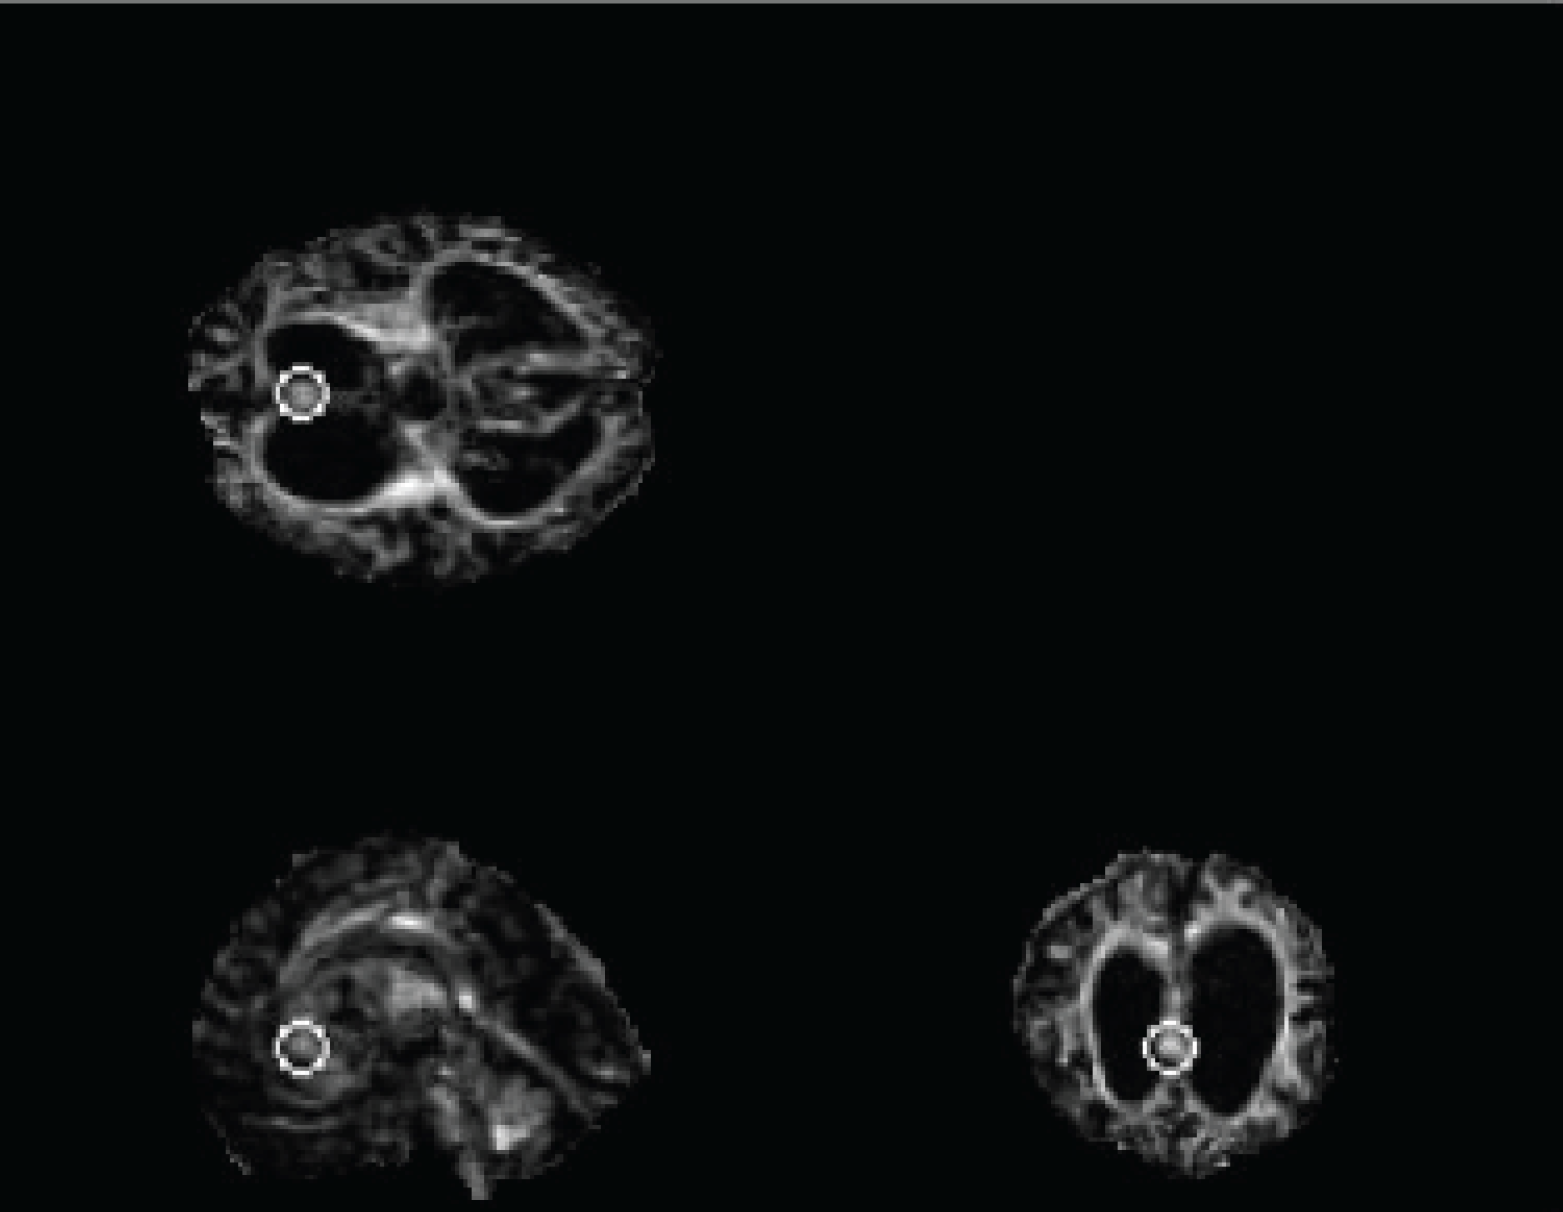
\includegraphics[height=0.33\textheight,width=0.49\columnwidth]{images/correspondence-b.png}\label{fig:corrB}}
    \caption{Example of one set of correspondence points.}
    \label{fig:corr}
\end{figure}

\subsection{Registration}
\label{subsec:registration}

\begin{figure}
    \centering
    \subfigure[Moving Image - Normal Control]{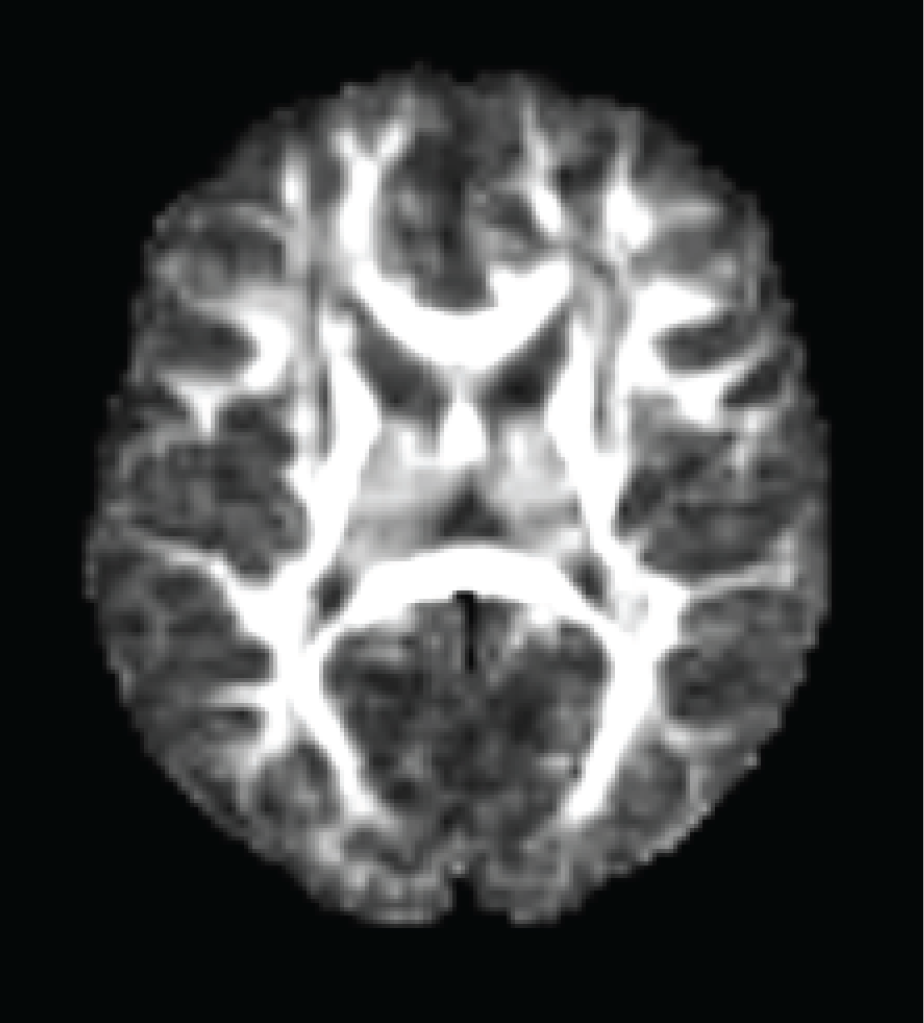
\includegraphics[height=0.20\textheight,width=0.30\textwidth]{images/RegResult-a.png}\label{fig:RegResultA}}
    \subfigure[Result of Demons]{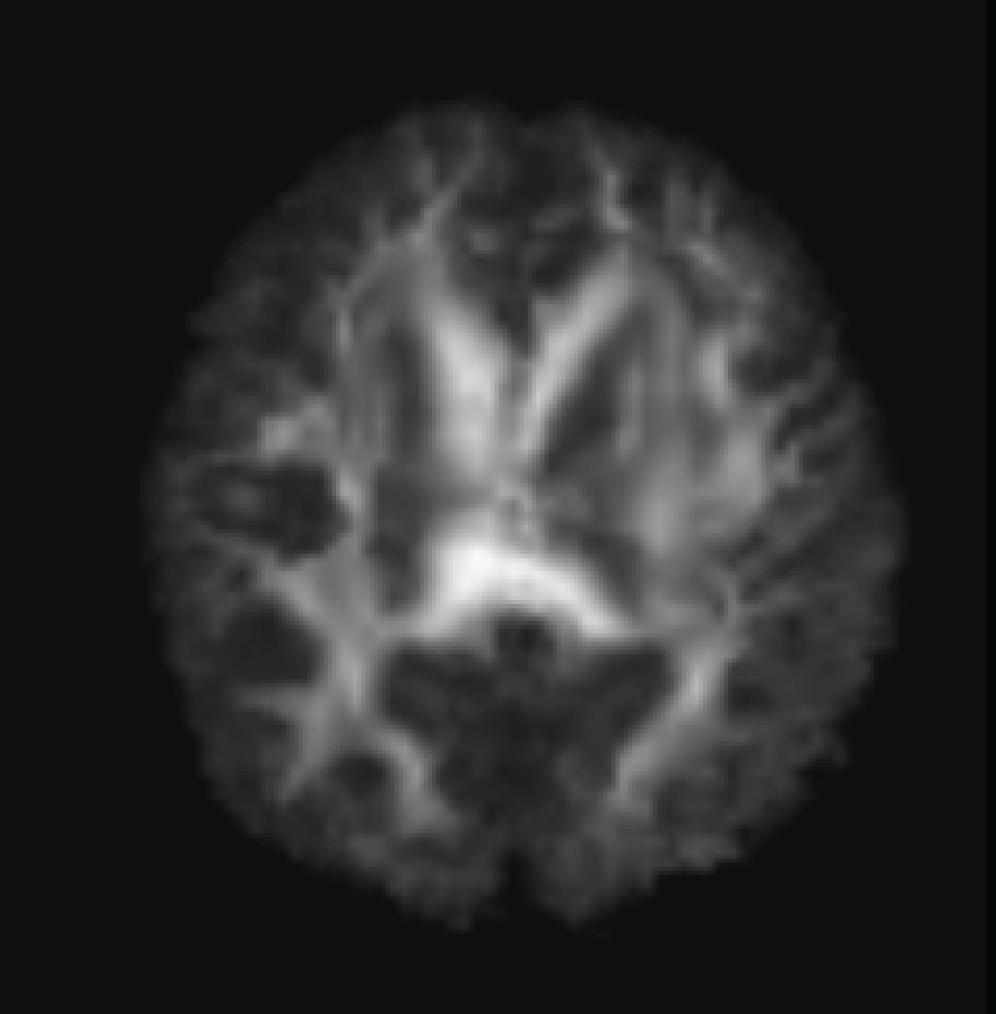
\includegraphics[height=0.20\textheight,width=0.30\textwidth]{images/RegResult-b.png}\label{fig:RegResultB}}
    \subfigure[Result of DTITK]{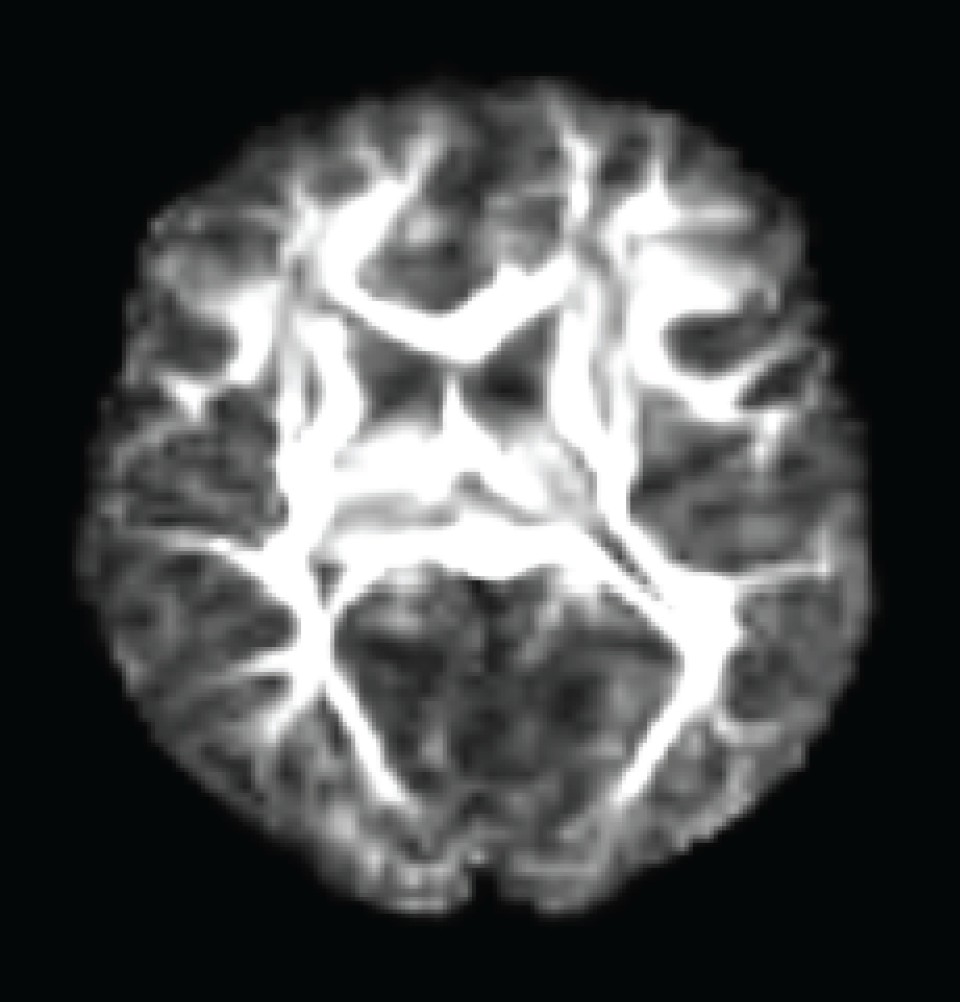
\includegraphics[height=0.20\textheight,width=0.30\textwidth]{images/RegResult-c.png}\label{fig:RegResultC}}
    \subfigure[Fixed Image - Krabbe]{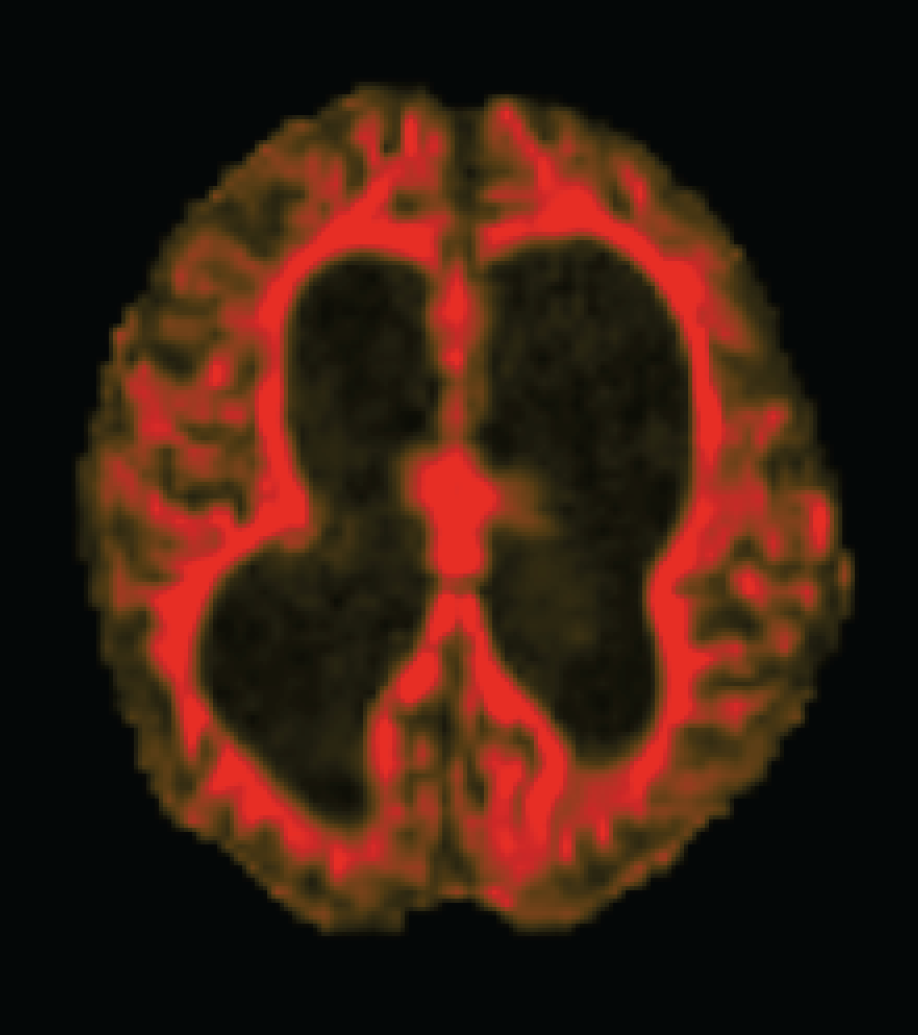
\includegraphics[height=0.20\textheight,width=0.30\textwidth]{images/RegResult-d.png}\label{fig:RegResultD}}
    \subfigure[Result of our method]{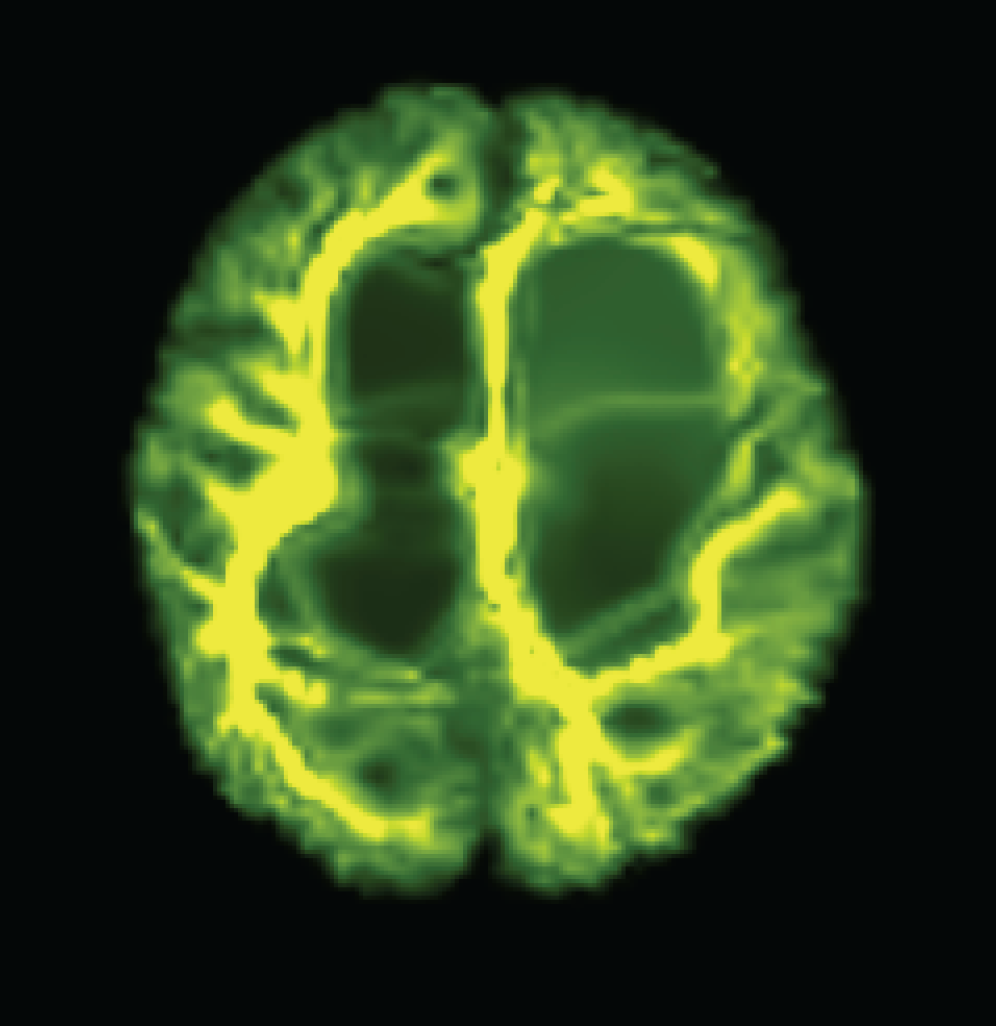
\includegraphics[height=0.20\textheight,width=0.30\textwidth]{images/RegResult-e.png}\label{fig:RegResultE}}
    \subfigure[Overlap of (d) and (e)]{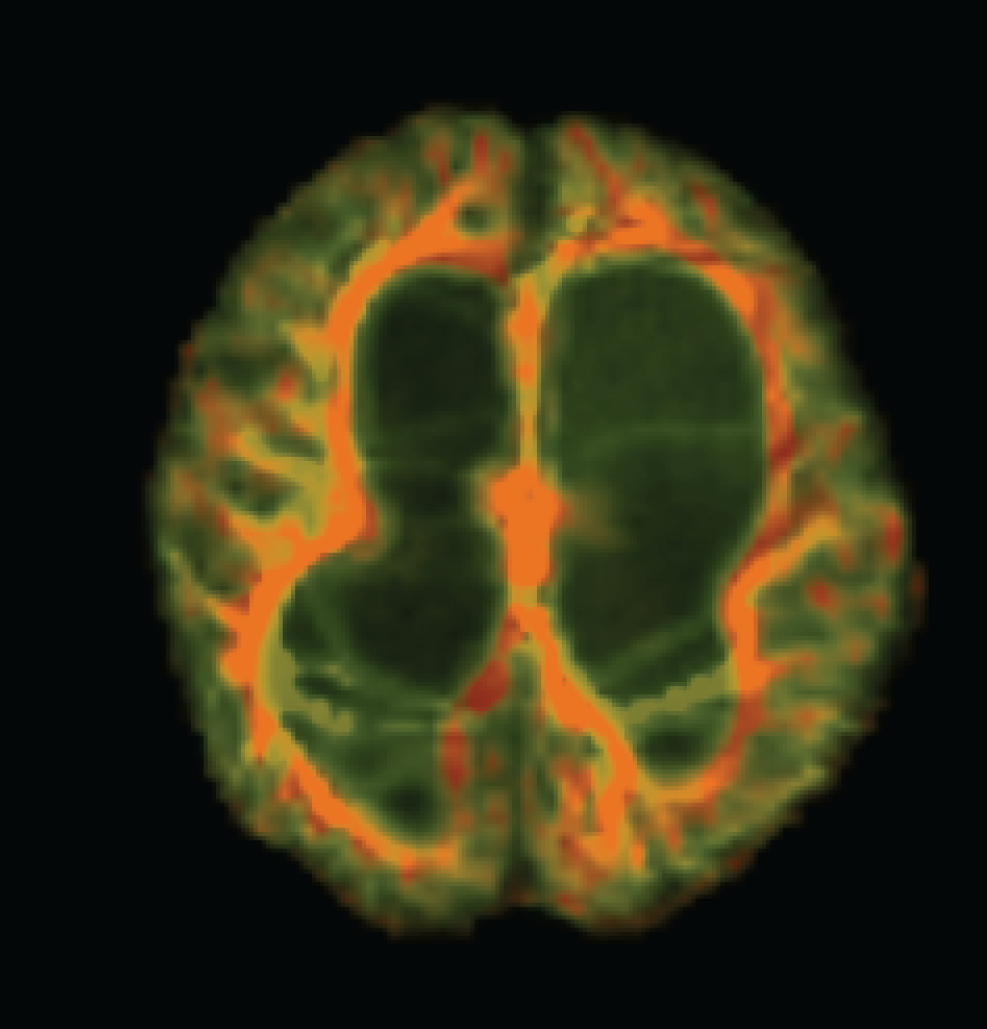
\includegraphics[height=0.20\textheight,width=0.30\textwidth]{images/RegResult-f.png}\label{fig:RegResultF}}
    \label{fig:regMatch}
    \caption{The figure shows the normal control FA map, the Krabbe subject FA map with the registration result with demons, DTITK and our proposed method.}
\end{figure}

Due to the large variation between the normal control and the subject with enlarged ventricles, a large deformation field is needed to register these images. Registration failed with the standard registration algorithms, including B-spline based (fnirt in FSL package), fluid based (fWarp in FSL), Demons (BRAINSDemonWarp in BRAINS) and also full tensor registration method DTITK within the DTI-Toolkit package. All the above methods failed to provide the large deformation required to register these images, particularly in the regions around the enlarged ventricles (figure \ref{fig:corr}).

To determine the large local deformation field, we first use the landmark correspondences to compute an initial deformation field. The computed landmarks are in general well distributed over the image and hence have the capability to estimate a global deformation field from these  local landmarks. We use  Gaussian radial basis functions (RBF) to determine the initial deformation field as implemented in the plastimatch registration toolkit. A Gaussian RBF decreases with growing distance from the landmark and the RBF asymptotically approaches zero. These properties along with the option of not selecting a polynomial part for RBF, give the desired advantage of decreasing global influence with higher distance from the landmarks. While we selected a straightforward landmark based deformation field generation in this work, there is lot of ongoing research in generating deformation fields from landmark points that potentially can improve the performance of our proposed registration approach. Once the deformation field is obtained, this field is used to initialize a deformable registration like diffeomorphic demons registration on intensity normalized FA images. The results of the combined fields - the point landmark deformation field and the demons deformation field on the FA images are presented in the next section.

\section{RESULTS}

The feature maps obtained from the fiber segments per voxel image and the normalized entropy image are shown in figure \ref{fig:featureMap}. For the fiber segments per voxel,  high intensity regions are expected and observed in regions of single fiber tracts and crossing fibers. For the entropy image, the high intensities are regions of dispersed fiber tracts (e.g., close to gray matter) and crossing fiber tracts (due to greater variation in fiber orientations) and lower intensities in unidirectional single fiber tracts (or in regions with lack of fiber tracts). The combination of  these two features results in a feature map highlighting crossing fibers and with lower intensities for the unidirectional single fiber situation. In comparison, FA maps cannot successfully highlight crossing fiber locations as these have often similar intensities as WM regions close to gray with largely dispersed fibers.

The deformation field obtained from the point correspondence provides the required initialization for standard registration algorithms. Since the feature maps have high intensity for the crossing fibers, this helps the point correspondence algorithm to determine good correspondences in spite of the large deformation. Figure \ref{fig:corr} shows an example of one set of correspondence points. Particularly in pathological cases where it is extremely difficult to even manually determine the landmarks because of the large abnormal deformation, our proposed method gives a considerable advantage.

To prove the potential of our method, we select a particular subject with abnormally large lateral ventricles. Figure 5 shows the FA images of the Krabbe case and the normal control and shows the results of Demons, DTITK and our proposed method. Clearly Demons and DTITK fail to produce the required deformation to push the corticospinal and the internal capsule tracts towards the necessary locations in the pathological subject. Also the figure shows the overlap of the target and image registered with our method to show the performance of our method. The regions in orange indicate the WM fiber tracts that are aligned successfully. From this overlap figure, a considerable success in registration is obtained for the major tracts - the genu, splenium and the internal capsule tracts.

Using the DWI volumes for the subject and the normal control, we generate the feature maps, as described in Section \ref{subsec:FeatureMap}. Figure \ref{fig:featureMap} shows the image representing the fiber segments per voxel, the normalized entropy and the combined final map. For the image representing the fiber segments per voxel,  high intensity regions are expected and observed in regions of single fiber tracts and crossing fibers, as both capture a large proportion of fiber segments. For the entropy image, the high intensities are regions of dispersed fiber tracts (e.g., close to gray matter) and crossing fiber tracts (due to greater variation in fiber orientations) and lower intensities in unidirectional single fiber tracts (or in regions with lack of fiber tracts). The combination of  these two features results in comparatively lower intensities the unidirectional single fiber situation as compared to crossing fiber situations. Furthermore, locations close or in gray matter display very low intensities in the combined map.  In comparison, FA maps cannot successfully highlight crossing fiber locations as these have often similar intensities as WM regions close to gray with largely dispersed fibers.

The combined feature map images for the subject and the normal control are then used as input to determine the point landmark correspondence. The point correspondences are used as inputs to the Gaussian RBF to determine the initial deformation field. This deformation field is used to initialize the demons algorithm applied on the subject and the normal control FA images. Figure 5 shows the FA images of the subject case (which is the fixed image) and the normal control deformed with the point landmark deformation field and the demons deformation field. Also the figure shows the overlap of these two images to show the performance of the registration. The regions in orange indicate the WM fiber tracts that are aligned successfully. From this overlap figure, a considerable success in registration is obtained for the major tracts - the genu, splenium and the internal capsule tracts.

The deformation field obtained from the point correspondence provides the required initialization for standard registration algorithms. Since the feature maps have high intensity for the crossing fibers, this helps the point correspondence algorithm to determine good correspondences in spite of the large deformation. Particularly in pathological cases where it is extremely difficult to even manually determine the landmarks because of the large abnormal deformation, our proposed method gives a considerable advantage.

To evaluate the registration, we use average regional matching criterion that is tailored to atlas based analysis methods. The orientation agreement between the principal eigenvectors of the source $e_{source}$ and the target $e_{target}$ weighted with the FA value of the target of each voxel of a particular region is the basis of this criterion. Regions of interest (ROI) on the Krabbe subject are defined representing major fiber tracts. For a ROI $r$, the average regional matching criterion is defined as: 
\begin{equation}
RegMatch_{r} = \frac{1}{N_{r}} \sum_{i=1}^{N_{r}} |e_{source}.e_{target}|.FA_{target}. N_{r}
\end{equation}
representing number of voxels in region $r$. The RegMatch percent values for the comparison of Demons, DTITK and our proposed method for three ROIs (100\% indicates perfect registration) are shown in Figure \ref{fig:Label_Table}. Considering the three ROIs, our proposed shows an improvement of 15.4\% over DTITK and 22.8\% over Demons method. 

\begin{figure}[htb]
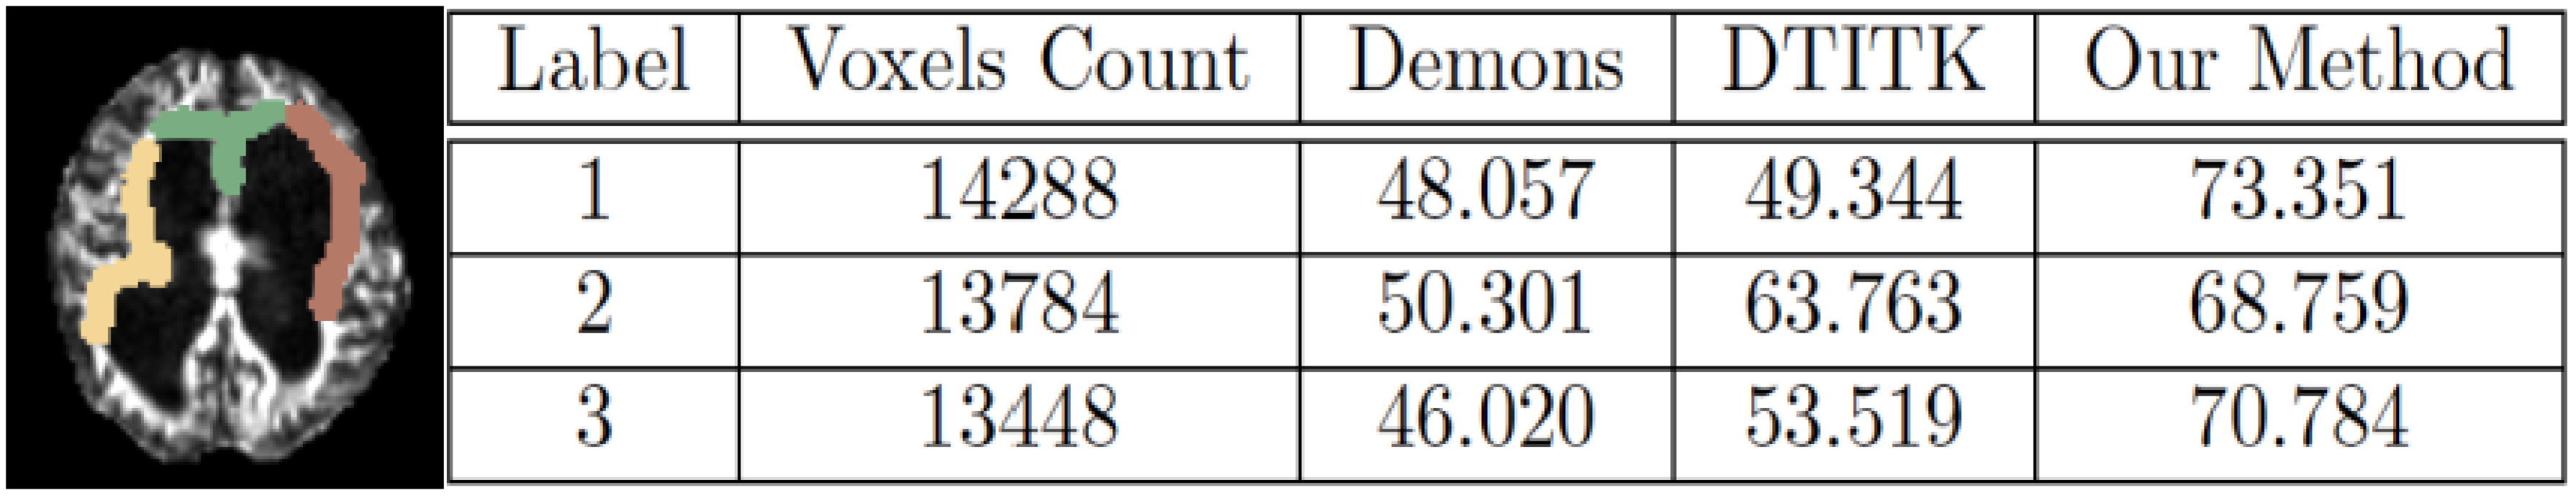
\includegraphics[width=1.0\columnwidth]{images/Table_LabelMap.png}
\centering
\caption{Labels on Krabbe case and percentage registration accuracy.}
\label{fig:Label_Table}
\end{figure}

\section{DISCUSSIONS and CONCLUSIONS}
In this paper, we have presented a novel, fully automatic pipeline to register images with large deformations, particularly subjects that are affected by WM demyelinating pathologies. The novel feature map computed is robust against variantions in WM fiber tract integrity and hence yields a good starting point to compute corresponding landmark points. The work presented here shows the potential of our pipeline to register highly deformed images as illustrated on a single, highly pathological case. We have applied the method to several more Krabbe cases with moderate to severely enlarged ventricles with similar success. Nevertheless, the presented registration pipeline is preliminary and several issues still need to be addressed, such as improving the stability of the landmark based deformation field computation against outliers/bad correspondences. For that purpose, we are currently working on incorporating weights for each landmark based on their correspondence quality score.

%
% ---- Bibliography ----
%
\bibliographystyle{splncs}
\bibliography{comp992}

\end{document}
